\documentclass[10pt]{article}
\usepackage[T1]{fontenc}
\usepackage{lmodern,amsmath,amssymb,graphicx,hyperref}
\usepackage[margin=0.8in]{geometry}
\setlength{\parindent}{0pt}\setlength{\parskip}{6pt}
\begin{document}
\begin{center}
{\Large Actual growing norm input budgets}\\[4pt]
Prime norm study, 14 November 2026\\
Source freeze \texttt{0a12a195c66785b5b8b4b4409ab0cc02ee991f64}
\end{center}

\textbf{Result.} The literal coefficient polynomial of the computed full
membership remainder obeys
\[
 \operatorname{wdeg}(R_j)\le 2\deg(P)-2j,
\]
with natural subtraction at zero. The theorem uses the actual multivariate
coefficient support, for every arity $a=h+2$, $h\in\mathbb N$.
PCC-20261114-253550/2c4a15; unsigned [pcc:unverified].
This is an input bound. It is not a bound on full iterated ideal closure.

\textbf{The actual family.} Over a field $K$, retain the variables $A_j$
($1\le j<a$) and $B_j$ ($0\le j\le a-2$), and public scalars
$\alpha,\beta,r,z$. Set
\begin{align*}
 D(X)&=X^a+\sum_{j=1}^{a-1}A_jX^j,&B(X)&=\sum_{j=0}^{a-2}B_jX^j,\\
 A(X)&=D(X)+zB(r)-D(r),&f(X)&=X^3+\alpha X+\beta,\\
 N(X)&=A(X)^2-f(X)B(X)^2,&U(X)&=N(X)\mathbin{\mathrm{divMonic}}(X-r),\\
 R(X)&=P(X)\mathbin{\mathrm{modMonic}}U(X).&&
\end{align*}
The public polynomial $P\in K[X]$ is arbitrary. A point-list nodal product
is a possible application; its generation is not assumed free.
The assigned weights are
$w(A_j)=2(a-j)$ and $w(B_j)=2a-3-2j$.
An explicit bijection identifies them with $1,\ldots,2a-2$;
PCC-20261114-cad062 [pcc:unverified].

\textbf{Support and incidence.} The actual norm is monic of degree $2a$;
its computed support $U$ is monic of degree $m=2a-1$.
These statements do not require a successful relation. If
$z^2=r^3+\alpha r+\beta$, then $(X-r)U=N$ by exact target incidence;
PCC-20261114-6c253b [pcc:unverified].

\textbf{Division proof.} A budget $d$ means
$w(e)+2j\le d$ for every exponent $e$ in the actual support of coefficient
$j$. The norm has budget $4a$, and $U$ has budget $2m$.
The generic theorem follows Mathlib's actual well-founded monic-division
recursion: each leading-term subtraction preserves the budget; the computed
quotient has budget $d-2m$, and the computed remainder has budget $d$.
A public degree-$B$ polynomial has budget $2B$, giving the displayed result.
No quotient, normal form, moment sequence or successful support is supplied.
PCC-20261114-3a3e7b/253550 [pcc:unverified].

\textbf{Exact original-chart binding.} At $h=1$, an equivalence renames
the coefficient polynomial ring to four indeterminates. The actual $A,B,N,U$
and full remainder equal the existing four-variable source expressions,
with weights $(4,2,3,1)$. This is a polynomial-ring identity, not equality
only on finite-field points. PCC-20261114-3a3330/69b0f2 [pcc:unverified].

\newpage
\begin{center}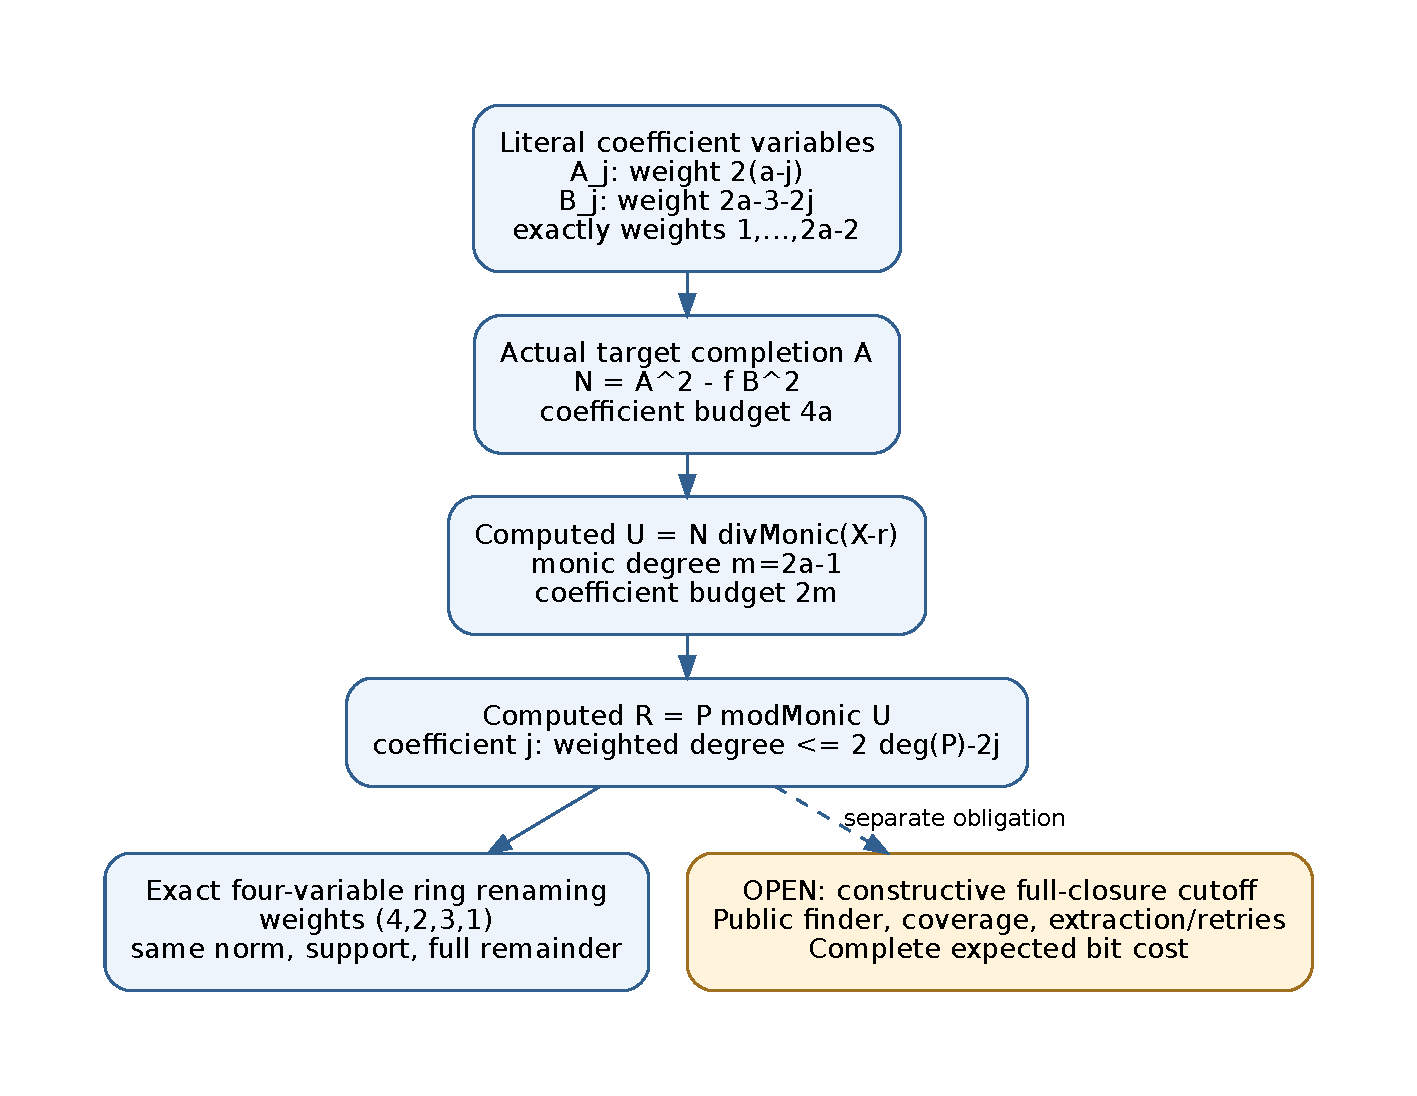
\includegraphics[height=0.55\textheight]{input.pdf}\end{center}
\textbf{Validation and provenance.} Forty authored theorems in:\\
\path{lean/NormInputBudget.lean}\\
\path{lean/NormGrowingInput.lean}.


Final source build006 exits0 without warnings; failed drafts and raw logs
are retained. Gate/fresh receipts and unsigned claim hashes are recorded
in the companion Markdown report. No signed verification is asserted.

Sources checked(KB): unavailable. Primary fallback read the actual
Mathlib support/weight lemmas and well-founded division recursion, plus
existing NormMembershipElimination, NormPoleTransport and NormTargetFiber.
Earlier weighted-GB and P1514/P1536 audits distinguish input grading from
regularity, available normal forms and efficient public construction.
No novelty claim is made for generic weighted division.

\textbf{Next dependency.} A constructive small full-closure cutoff for
this growing family is still required. The prior finite weighted count can
price a given cutoff; this input bound does not supply that cutoff. Public
base coverage, signed output, field extraction, failed attempts and complete
expected bit cost remain charged obligations. No normalized-row degree29
or original $W_{\rm new}=W_{\rm base}+CH$ jet map is established here.
No solver, native fixture, paid job, timing measurement or Python cryptomath
was run. Canonical performance graphs stay unchanged.
\end{document}
